
\documentclass[border=10pt,varwidth]{standalone}
\usepackage[left=25mm,right=25mm,top=25mm,bottom=25mm]{geometry}
\usepackage[utf8]{inputenc}
\usepackage[T1]{fontenc}
\usepackage{times}
\usepackage{geometry}
\usepackage{amsmath}
\usepackage{amssymb}
\usepackage{mathrsfs}
\usepackage{amsfonts}
\usepackage{amsthm}
\usepackage{lipsum}
\usepackage{amscd}
\usepackage{graphicx}
\usepackage{fancyhdr}
\usepackage{textcomp}
\usepackage{pgfplots}
\usepackage{txfonts}
\usepackage[all]{xy}
\usepackage{paralist}
\usepackage[colorlinks=true]{hyperref}
\usepackage{array}
\usepackage{tikz}
\usepackage{slashed}
\usepackage{pdfpages}
\usepackage{cite}
\usepackage{url}
\usepackage{amsmath,amsfonts,amssymb}
\usepackage{tikz}
\usepackage{pgfplotstable}
\usetikzlibrary{arrows,matrix,positioning}
\usetikzlibrary{overlay-beamer-styles}
\usetikzlibrary{matrix.skeleton}
\usetikzlibrary{automata,positioning}
\usetikzlibrary{decorations.text}
\usepackage{listings}
\usepackage{multirow}
\usepackage{color}

\begin{document}

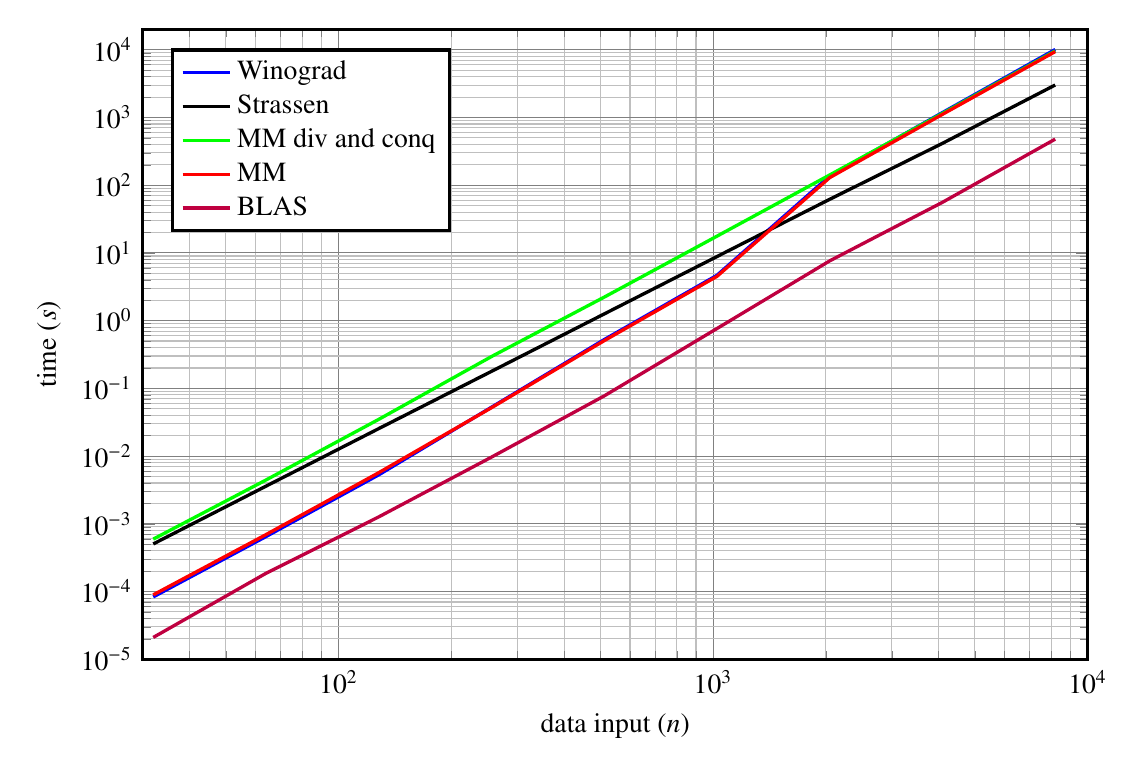
\begin{tikzpicture}
\begin{axis}[
xmode=log, ymode=log,
xmin=30, xmax=10000,
ymin=1e-5, ymax=2e4,
grid=both,
major grid style={black!50},
xlabel = data input ($n$),
ylabel = {time ($s$)},
legend pos=north west,
very thick,
scale only axis=true,
width=12cm, height=8cm,
       log basis x={10},
       legend cell align={left}
]
\addlegendentry{Winograd}
\addplot[    color=blue,
        error bars/.cd, y dir=both, y explicit,
] coordinates {
%(2,1e-07)
%(4,5e-07)
%(8,2.0000000000000003e-06)
%(16,1.1999999999999999e-05)
(32,8.329999999999999e-05)
(64,0.0006479)
(128,0.0052873)
(256,0.052674599999999995)
(512,0.5249752000000001)
(1024,4.671161)
(2048,136.6769777)
(4096,1179.261048)
(8192,10071.512655)
};
\addlegendentry{Strassen}
\addplot [    color=black,
]coordinates {
%(2,1e-07)
%(4,2.1e-06)
%(8,1.13e-05)
%(16,7.07e-05)
(32,0.0005041)
(64,0.003596)
(128,0.0254481)
(256,0.1781817)
(512,1.2555)
(1024,8.8302371)
(2048,61.9018691)
(4096,414.648901)
(8192,3014.235467)
};

\addlegendentry{MM div and conq}
\addplot[    color=green,
] coordinates {
%(2,3e-07)
%(4,1.1e-06)
%(8,8.6e-06)
%(16,7.819999999999999e-05)
(32,0.0005940000000000001)
(64,0.0044339)
(128,0.0348443)
(256,0.29484730000000003)
(512,2.2228507)
(1024,17.659234500000004)
(2048,141.6103936)
(4096,1147.106865)
(8192,9606.402522)
};

\addlegendentry{MM}
\addplot [    color=red,
]coordinates {
%(2,0.0)
%(4,3e-07)
%(8,1.8000000000000001e-06)
%(16,1.1999999999999999e-05)
(32,8.93e-05)
(64,0.0006923)
(128,0.0056842)
(256,0.051771500000000005)
(512,0.5062468000000001)
(1024,4.5048086)
(2048,129.2894619)
(4096,1111.312696)
(8192,9376.173434)
};
\addlegendentry{BLAS}
\addplot[    color=purple,
] coordinates {
%(2,1e-07)
%(4,0.0)
%(8,1e-07)
%(16,3.9e-06)
(32,2.1000000000000002e-05)
(64,0.00018580000000000002)
(128,0.0012649)
(256,0.0096489)
(512,0.0773765)
(1024,0.7643868)
(2048,7.6320993999999995)
(4096,55.845038)
(8192,478.429957)
};
\end{axis}
\end{tikzpicture}

\end{document}
